\documentclass{article}

\PassOptionsToPackage{numbers, compress}{natbib}
\usepackage[preprint]{neurips_2025}

\usepackage[utf8]{inputenc}
\usepackage[T1]{fontenc}
\usepackage{hyperref}
\usepackage{url}
\usepackage{booktabs}
\usepackage{amsfonts}
\usepackage{amsmath}
\usepackage{amssymb}
\usepackage{amsthm}
\usepackage{microtype}
\usepackage{xcolor}
\usepackage{graphicx}
\usepackage{multirow}
\usepackage{array}
\usepackage{float}
\renewcommand{\ttdefault}{lmtt}
\floatstyle{ruled}
\newfloat{algorithm}{t}{loa}
\floatname{algorithm}{Algorithm}

\hypersetup{
  colorlinks=true,
  linkcolor=blue!60!black,
  citecolor=green!45!black,
  urlcolor=blue!65!black
}

\newtheorem{proposition}{Proposition}
\newtheorem{remark}{Remark}

\newcommand{\EVR}{\mathrm{EV}_R}
\newcommand{\FeeR}{\mathrm{Fee}_R}
\newcommand{\StdR}{\mathrm{Std}_R}
\newcommand{\RR}{\mathrm{RR}}
\newcommand{\TP}{\mathrm{TP}}
\newcommand{\SL}{\mathrm{SL}}
\newcommand{\ATR}{\mathrm{ATR}}
\newcommand{\MAE}{\mathrm{MAE}}
\newcommand{\logit}{\operatorname{logit}}
\newcommand{\PF}{\mathrm{PF}}

\title{Beyond Next-Candle Prediction: Leakage-Free Multi-R:R Expected-Value Learning and the Role of Market Time Zones Across Crypto, Forex, and Equity Indices}

\author{
  Benyamin Eslami \hspace{1.5em} Joshua Burk \hspace{1.5em} Byron Fisher \hspace{1.5em} Joshua Oliver \\
  School of Electrical Engineering and Computer Science \\
  Washington State University \\
  Pullman, WA 99164 \\
}

\begin{document}

\maketitle

\begin{abstract}
Many machine learning papers treat financial trading as next-candle price prediction or binary up/down classification, often reporting $80\%$--$97\%$ accuracy or $R^2 > 0.90$. Under realistic trading fees and strict time-ordered testing, however, next-candle forecasting rarely makes money. We identify four direct reasons: (1) fees eat small single-bar moves, (2) one-bar predictions do not match multi-hour trade horizons, (3) direction accuracy ignores intrabar stop-outs and payoff asymmetry, and (4) probabilities drift when market regimes change. First, we demonstrate these problems with a leakage-free three-model consensus (\texttt{XGBoost}, \texttt{LSTM}, and Logistic Regression) on $59{,}904$ hourly Bitcoin candles ($2020$--$2026$). Even though the ensemble beats a coin flip ($53.41\%$ overall accuracy, $59.05\%$ at confidence $\ge 0.60$, $p < 0.001$), mapping those $1$-hour probabilities onto $24$--$48$h bracket trades produces $0 / 11{,}979$ positive expected-value trades. Second, we reformulate trading as \emph{cost-aware multi-$\RR$ barrier probability estimation} using a strictly purged two-stage walk-forward pipeline with rolling $2$-year ATR-normalized stop-losses, factorized directional and timeout heads, a lagged $60$-day probability recalibrator, a Per-Trade Sharpe selector ($S = \EVR / \StdR$), a universal fee limit ($\FeeR \le 0.05R$), and an automatic stand-down rule. Third, we test this exact pipeline across nine liquid symbols from three asset classes ($2025$--$2026$ out-of-sample): two cryptocurrencies (\texttt{BTC}, \texttt{ETH}), five G10 Forex pairs (\texttt{EURUSD}, \texttt{GBPUSD}, \texttt{JPYUSD}, \texttt{AUDUSD}, \texttt{CADUSD}), and two US equity indices (\texttt{SPX}, \texttt{NDX}). Our key finding is that \textbf{even when a model produces accurate, well-calibrated signals, the market time zone has a major impact on strategy profit}. On Forex, evaluating on $100\%$ continuous real candles with entry-only session masking shows that the Asian session ($00{:}00$--$09{:}00$ UTC) behaves like coin-flip noise ($\mathrm{AUC} = 0.513$, $-42.28R$ on Fixed-ATR), whereas the New York session ($12{:}00$--$21{:}00$ UTC) raises AUC on all five pairs ($\mathrm{AUC} = 0.643$) and earns $+16.49R$ with zero losing pairs, and the London session ($07{:}00$--$16{:}00$ UTC) earns $+18.32R$ on Learned-SL (led by \texttt{JPYUSD} $+16.40R$, $\PF = 2.95$, $1.84\%$ drawdown). On US equity indices, masking entries to New York Regular Trading Hours ($09{:}30$--$16{:}00$ ET) removes a $-27.05R$ overnight \texttt{NDX} loss cleanly ($0.00R$ on \texttt{SPX}, $-0.20R$ to $0.00R$ on \texttt{NDX}). On 24/7 crypto, continuous 24/7 trading (\texttt{ETH} $+17.23R$ Fixed-ATR; \texttt{BTC} $+4.25R$ and \texttt{ETH} $+5.29R$ Learned-SL) outperforms weekday-only masking (\texttt{ETH} $+11.04R$, \texttt{BTC} $0.00R$ to $-4.36R$). Finally, we expose a serious backtesting trap---naive CSV row deletion creates fake gap profits and broken indicators---and show how continuous-candle entry masking solves it completely.
\end{abstract}

% ==============================================================================
\section{Introduction}
\label{sec:intro}

Predicting financial markets with machine learning is difficult because liquid markets quickly adjust to public price information~\citep{Fama1970}. Any remaining short-term edge comes mainly from temporary order-flow imbalances~\citep{Kyle1985}, liquidity costs~\citep{Amihud2002}, and recurring trading-session patterns. Despite this reality, many papers and public code projects still report $R^2 > 0.92$ on raw price levels~\citep{Islam2025IJAES} or $80\%$--$90\%$ directional accuracy~\citep{Bansal2022}. When strict time-ordered testing is enforced across many markets without data leakage, directional accuracy drops to roughly $51\%$~\citep{Bustos2025}.

More importantly, \emph{even a clean, leakage-free model that beats a coin flip on next-candle direction is usually unprofitable to trade}. Across our experiments from $2020$ to $2026$, we observe four direct reasons why next-candle prediction fails:

\begin{enumerate}
    \item \textbf{Fees Eat Small Moves.} On $15$-minute or $1$-hour bars, a typical candle moves only $0.05\%$--$0.40\%$. Under symmetric $1{:}1$ exits, round-trip trading fees $2c$ take up a large share of risked capital: in $R$-multiples, fee drag is $\FeeR \approx 2c / \delta_s$ (Section~\ref{sec:theory}, Figure~\ref{fig:ev_theory}a). When stops become too tight during quiet hours, fees erase small statistical edges.
    \item \textbf{Prediction Horizon Does Not Match Trade Horizon.} Many systems train on $1$-bar labels ($C_{t+1} > C_t$) and then use those probabilities to enter multi-hour Stop-Loss ($\SL$) and Take-Profit ($\TP$) trades. In Section~\ref{sec:phase1_results}, we show that applying a well-calibrated $1$-hour consensus model ($53.41\%$ accuracy, $p<0.001$) to $24$--$48$h brackets rejects all $11{,}979 / 11{,}979$ test hours ($0$ trades). Short-term order-flow signals fade long before wide brackets finish.
    \item \textbf{Direction Accuracy Ignores Trade Path and Payoff Size.} Financial returns have heavy tails and sharp intrabar wicks. Predicting only $\operatorname{sign}(C_{t+1} - C_t)$ ignores whether price first hits the stop-loss before moving into profit, and treats a tiny $+0.02\%$ bar the same as a $+2.5\%$ breakout. With asymmetric targets ($\RR \in [2.0, 4.0]$), a strategy can profit with only a $30\%$--$35\%$ win rate if it accurately estimates \emph{which barrier hits first}~\citep{LopezDePrado2018}.
    \item \textbf{Market Time Zones and Regimes Change Probability Behavior.} Even calibrated models drift when volatility or liquidity changes. More sharply, we discover in Section~\ref{sec:timezone_results} that the \emph{exact same model} can earn strong profits in one global trading session and lose heavily in another, purely because volatility, liquidity, and macro news cluster in specific hours of the day.
\end{enumerate}

\paragraph{Main Contributions.} We build and test a clean, leakage-free trading research system across nine symbols and three asset classes:
\begin{itemize}
    \item \textbf{Phase-1 Next-Candle Diagnostic (\texttt{BTC 1h}, Section~\ref{sec:phase1_results}):} We test a three-model consensus (\texttt{XGBoost}, \texttt{LSTM}, Logistic Regression) on $59{,}904$ hourly Bitcoin candles ($2020$--$2026$), measuring real directional accuracy ($53.41\%$ overall, $59.05\%$ at high confidence), declining accuracy over time, and why $1$-hour signals fail on multi-hour brackets.
    \item \textbf{Cost-Aware Multi-$\RR$ Expected-Value Framework (Sections~\ref{sec:theory}--\ref{sec:models}):} We derive exact fee-adjusted expected value $\EVR$, break-even hit rate $p_{\mathrm{be}}$, the scale-free commission rule $\FeeR \le 0.05R$, and the Per-Trade Sharpe selector $S = \EVR / \StdR$. We train factorized directional and timeout heads inside a $4$-way purged walk-forward loop with fresh rolling $2$-year Stage-1 stops, $60$-day lagged recalibration, and automatic stand-down when validation profit is non-positive.
    \item \textbf{Payoff Audit and Simple Baseline Test (\texttt{BTC} \& \texttt{ETH}, Section~\ref{sec:audit}):} We show that crediting timeout payoffs inside the entry gate hurts performance because timeout timing is much easier to predict ($\mathrm{AUC} \approx 0.69$--$0.74$) than price direction ($\mathrm{AUC} \approx 0.55$--$0.59$). Using a conservative entry gate restores profit (\texttt{BTC} $+4.25R$, \texttt{ETH} $+5.29R$), and a simpler $2$-head Fixed-ATR ($1.5\,\ATR$, $2.5{:}1$) model removes $10$-head selection noise to earn $+17.23R$ on \texttt{ETH} equally across bull ($+8.57R$) and bear ($+8.66R$) periods.
    \item \textbf{Cross-Asset Time Zone Study and Phantom-Gap Fix (Sections~\ref{sec:data} \& \ref{sec:timezone_results}):} Across \texttt{BTC}, \texttt{ETH}, five G10 Forex pairs (\texttt{EURUSD}, \texttt{GBPUSD}, \texttt{JPYUSD}, \texttt{AUDUSD}, \texttt{CADUSD}), and two US equity indices (\texttt{SPX}, \texttt{NDX}), we prove that trading time zone strongly controls profitability even when signals are accurate. We also document \emph{Session-Slicing Phantom Gap Bias} and fix it by keeping $100\%$ of continuous candles while masking only training, calibration, and new entries.
\end{itemize}

% ==============================================================================
\section{Related Work and Common Mistakes in Financial ML}
\label{sec:related}

Past studies on machine learning for market prediction vary widely in testing rigor. \citet{Bansal2022} test KNN, Linear Regression, SVR, Decision Trees, and LSTM on $12$ Indian stocks ($2015$--$2021$) using price-level error metrics, but use a $99{:}1$ split with only $8$ test days per stock; even their best LSTM gets negative out-of-sample $R^2 = -0.11$. \citet{Islam2025IJAES} add liquidity features inspired by \citet{Kyle1985} and \citet{Amihud2002} to predict \texttt{XRP/USDT} price levels and report $R^2 = 0.9295$. High price-level $R^2$ occurs mostly because tomorrow's price is close to today's price ($P_{t+1} \approx P_t$), not because the model can predict profitable price changes.

When studies switch to directional classification, true accuracy is much lower. \citet{Islam2025JoE} test Logistic Regression ($56.03\%$), Random Forest ($46.30\%$), and XGBoost ($45.14\%$) on $257$ crypto test samples, showing that simple regularized linear models often beat complex tree ensembles on noisy targets. Most clearly, \citet{Bustos2025} evaluate seven model families across $55$ global stock markets and $65$ two-month time-ordered test windows ($2011$--$2022$). Average leakage-free accuracy stays near $51\%$ for every model family: SVM ($51.64\%$), Gradient Boosting ($51.61\%$), Neural Networks ($51.60\%$), Random Forest ($51.22\%$), Logistic Regression ($51.17\%$), Naive Bayes ($51.14\%$), and LSTM ($50.95\%$).

Reviewing public financial-ML repositories reveals five repeated engineering errors that cause inflated results: (1) randomly shuffling time-series rows before splitting, (2) scaling features using the entire dataset before splitting, (3) merging higher-timeframe candles by open time instead of close time (leaking future prices), (4) omitting purge gaps between train and test splits when labels look ahead~\citep{LopezDePrado2018}, and (5) ignoring fees or assuming take-profit hits before stop-loss on ambiguous bars. In addition, tabular ML benchmarks~\citep{Grinsztajn2022} show that regularized gradient-boosted trees~\citep{Chen2016} match or beat deep sequence models~\citep{Hochreiter1997} on medium-sized tabular signals, while probability calibration~\citep{Platt1999, Guo2017} and overfitting checks~\citep{Bailey2014} are essential when probabilities control trade sizing. In this paper, we also uncover a sixth common error: \emph{deleting off-session rows from continuous price files before backtesting}, which creates fake gap fills and breaks rolling indicators.

% ==============================================================================
\section{Problem Formulation and Fee-Adjusted Expected-Value Theory}
\label{sec:theory}

Let $\{(O_t, H_t, L_t, C_t, V_t, \mathbf{m}_t)\}_{t=1}^T$ be a time-ordered candlestick series together with strictly causal market features $\mathbf{m}_t$. At the close of bar $t$, the model sees feature vector $\mathbf{x}_t \in \mathbb{R}^d$ and decides whether to place a bracket trade at the \emph{next} bar's open price $e = O_{t+1}$. Each candidate trade has direction $s \in \{+1, -1\}$ (Long or Short), relative stop-loss width $\delta_s(t) = \mathrm{sl\_pct}_s(t) > 0$, target reward-to-risk ratio $r \in \mathcal{R} = \{2.0, 2.5, 3.0, 3.5, 4.0\}$, and maximum holding length $H = \mathrm{max\_bars}$ ($32$ bars $= 8$ hours on $15\text{m}$ data).

The stop-loss and take-profit prices are:
\begin{equation}
  \SL = e \cdot (1 - s\,\delta_s), \qquad
  \TP = e \cdot (1 + s\,r\,\delta_s), \qquad
  \text{so that } \frac{|\TP - e|}{|\SL - e|} = r.
  \label{eq:barriers}
\end{equation}
Over the next $H$ real continuous bars $t+1, \dots, t+H$, each bracket has three possible outcomes: \texttt{TP} (take-profit touched first), \texttt{SL} (stop-loss touched first), or \texttt{TIMEOUT} (neither barrier touched, so the trade closes at $C_{t+H}$). Whenever a single candle spans both $\SL$ and $\TP$, we always assume $\SL$ hits first (conservative tie-breaking).

\subsection{Exact Fee-Adjusted Expected Value and Conservative Gating}

Let $c \ge 0$ be the one-way trading fee rate charged on both entry and exit notional value. Under equal-risk sizing, one unit of initial risk ($1R$) equals the stop distance $D_{\SL} = |e - \SL| = e\,\delta_s$ per unit of quantity $q$. If a trade wins at $\TP$, gross gain is $+r\,D_{\SL}$ and round-trip fee is $c(e + \TP)$. If it loses at $\SL$, gross loss is $-D_{\SL}$ and round-trip fee is $c(e + \SL)$. Dividing by $D_{\SL}$ gives the conservative lower-bound expected value in $R$-multiples (treating both $\SL$ and $\mathrm{TIMEOUT}$ as $-1R$):
\begin{equation}
  \EVR^{\mathrm{cons}}(e, \TP, \SL, p, c)
  \;=\; \left(\frac{|\TP - e|}{|\SL - e|} + 1\right) p \;-\; 1
  \;-\; \frac{p \cdot c(\TP + e) + (1 - p) \cdot c(e + \SL)}{|e - \SL|}.
  \label{eq:ev_exact}
\end{equation}
Substituting Eq.~\eqref{eq:barriers} writes Eq.~\eqref{eq:ev_exact} directly in terms of $(s, r, \delta_s, p, c)$:
\begin{equation}
  \EVR^{\mathrm{cons}}(s, r, \delta_s, p, c)
  \;=\; (r + 1)p - 1 - \underbrace{\frac{c\bigl[2 + s\,\delta_s(p\,r - (1-p))\bigr]}{\delta_s}}_{\FeeR(s, r, \delta_s, p, c)}.
  \label{eq:ev_simplified}
\end{equation}
Setting $\EVR^{\mathrm{cons}} = 0$ gives the exact fee-adjusted break-even hit rate:
\begin{equation}
  p_{\mathrm{be}}(e, \TP, \SL, c)
  \;=\; \frac{|e - \SL| + c(e + \SL)}{|\TP - e| + |e - \SL| - c(\TP - \SL)}
  \;\approx\; \frac{1 + 2c/\delta_s}{r + 1}.
  \label{eq:p_be}
\end{equation}

\paragraph{Exact Three-Outcome Expected Value vs.\ Conservative Entry Gate.}
Because unresolved trades close at market price $C_{t+H}$ after $H$ bars rather than losing $-1R$, the simulator's true three-outcome expected value (ignoring gap slippage) is:
\begin{equation}
  \EVR^{\mathrm{exact}}
  \;=\; p_{\TP}\,r - p_{\SL} + p_{\mathrm{TO}}\,\mathbb{E}[R_{\mathrm{TO}} \mid \mathrm{TO}, \mathbf{x}_t] - \mathbb{E}[\FeeR],
  \label{eq:ev_3outcome}
\end{equation}
where the gap between exact and conservative expected value is
\begin{equation}
  \EVR^{\mathrm{exact}} - \EVR^{\mathrm{cons}}
  \;=\; p_{\mathrm{TO}}\cdot\bigl(1 + \mathbb{E}[R_{\mathrm{TO}} \mid \mathrm{TO}, \mathbf{x}_t]\bigr) \;\ge\; 0.
  \label{eq:ev_gap}
\end{equation}
Because asymmetric brackets ($\SL = -1R, \TP = +r$) knock out downward paths early at $\SL$, surviving timeouts have positive average payoff ($\mathbb{E}[R_{\mathrm{TO}} \mid \mathrm{TO}] \approx +0.3R$ to $+1.0R$). In Section~\ref{sec:audit}, we test Eq.~\eqref{eq:ev_3outcome} directly against Eq.~\eqref{eq:ev_exact}. Surprisingly, crediting timeouts inside the entry gate fails badly ($-4.7R$ to $-89.7R$) because timeout probability $p_{\mathrm{TO}}$ is much easier to predict ($\mathrm{AUC} \approx 0.69$--$0.74$) than price direction ($\mathrm{AUC} \approx 0.55$--$0.59$). When the gate credits timeouts, it fills up with slow, low-edge trades. Keeping the conservative gate $\EVR^{\mathrm{cons}}$ acts as a simple safety filter that requires genuine directional edge.

\begin{remark}[Why a $30\%$--$35\%$ Win Rate Can Still Be Profitable]
\label{rem:asymmetric}
Before fees, break-even win rates for $r \in \{2.0, 2.5, 3.0, 3.5, 4.0\}$ are $p_{\mathrm{be}} \in \{33.3\%, 28.6\%, 25.0\%, 22.2\%, 20.0\%\}$. A strategy with a $33.3\%$ win rate at $2.5{:}1$ (our \texttt{ETH} Fixed-ATR result) earns $+17.23R$ ($\PF = 1.12$) because winners pay $+2.5R$ while losers stop at $-1R$.
\end{remark}

\subsection{Universal Micro-Stop Fee Gate Across Asset Classes}

From Eq.~\eqref{eq:ev_simplified}, round-trip commission drag in $R$-multiples is approximately
\begin{equation}
  \FeeR \;\approx\; \frac{2c \cdot e}{|e - \SL|} \;=\; \frac{2c}{\delta_s}.
  \label{eq:fee_r}
\end{equation}
Different asset classes have very different intraday volatility and trading costs. A fixed percentage stop floor (such as $\delta_s \ge 0.40\%$) works for Bitcoin but would block $99.5\%$ of $15$-minute Forex candles (where median $\ATR\%$ is only $0.05\%$--$0.08\%$). Instead, we apply one universal cost rule across every symbol:
\begin{equation}
  \text{Reject trade if } \quad \FeeR(t) = \frac{2c}{\delta_s(t)} \;>\; 0.05R
  \quad\Longleftrightarrow\quad
  \delta_s(t) < 40c.
  \label{eq:fee_gate}
\end{equation}
Figure~\ref{fig:ev_theory}(a) shows how Eq.~\eqref{eq:fee_gate} automatically scales with each asset class's realistic institutional cost:
\begin{itemize}
    \item \textbf{Crypto (\texttt{BTC}, \texttt{ETH}):} Binance VIP/maker cost $c = 0.00010$ ($1.0\text{ bp}$/side) $\Rightarrow$ blocks stops below $0.40\%$.
    \item \textbf{US Equity Indices (\texttt{SPX}, \texttt{NDX}):} CME E-mini futures cost $c = 0.00005$ ($0.5\text{ bp}$/side) $\Rightarrow$ blocks stops below $0.20\%$.
    \item \textbf{G10 Forex (\texttt{EURUSD}--\texttt{CADUSD}):} Institutional ECN cost $c = 0.00002$ ($0.2\text{ bp}$/side, $\approx 0.4\text{ pips}$ round-trip) $\Rightarrow$ blocks stops below $0.08\%$ ($\approx 8\text{ pips}$).
\end{itemize}
In all three asset classes, this single rule keeps round-trip fees at or below $5\%$ of risked capital and automatically skips quiet, low-volatility micro-stops.

\begin{figure}[t]
  \centering
  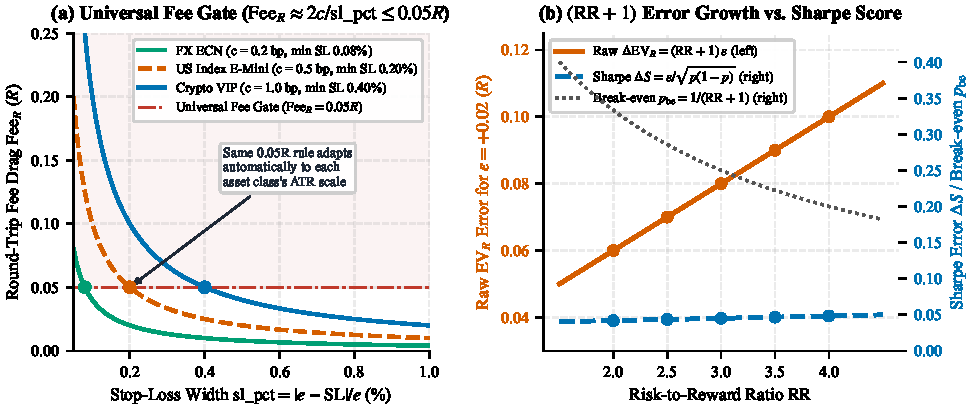
\includegraphics[width=\textwidth]{figures/fig2_ev_and_fee_theory.pdf}
  \caption{\textbf{Fee drag and calibration-error geometry.} \textbf{(a)} Round-trip fee drag $\FeeR \approx 2c/\mathrm{sl\_pct}$ across all three asset-class fee tiers; one rule ($\FeeR \le 0.05R$) automatically adapts minimum stop width to Forex ($0.08\%$), US equity indices ($0.20\%$), and crypto ($0.40\%$). \textbf{(b)} A $+2\text{ pp}$ probability overestimate inflates raw $\EVR$ linearly by $(\RR+1)\epsilon$, biasing selection toward noisy $4{:}1$ targets, whereas Per-Trade Sharpe $S = \EVR / \StdR$ removes the $(\RR+1)$ multiplier.}
  \label{fig:ev_theory}
\end{figure}

\subsection{Removing \texorpdfstring{$(\RR+1)$}{(RR+1)} Calibration Noise with Per-Trade Sharpe Selection}

When choosing the best trade among $10$ candidate heads, simply picking $\arg\max_{s,r} \EVR(s,r)$ favors noisy high-$\RR$ heads.

\begin{proposition}[Calibration Error Growth and Sharpe Cancellation]
\label{prop:sharpe}
If an estimated probability overshoots the true hit rate by $\epsilon > 0$ ($\hat{p}_{s,r} = p_{s,r} + \epsilon$), the induced error in raw $\EVR$ grows linearly with $r$:
\begin{equation}
  \Delta \EVR(r) \;=\; \EVR(\hat{p}_{s,r}) - \EVR(p_{s,r}) \;\approx\; (r + 1)\,\epsilon.
  \label{eq:ev_noise}
\end{equation}
Modeling a single trade's gross payoff $R_{\mathrm{trade}} \in \{+r, -1\}$ as a scaled Bernoulli variable with standard deviation $\StdR(r, \hat{p}) = (r + 1)\sqrt{\hat{p}(1-\hat{p})}$, the \emph{Per-Trade Sharpe Score}
\begin{equation}
  S(s, r) \;=\; \frac{\EVR^{\mathrm{cons}}(s, r, \delta_s, \hat{p}_{s,r}, c)}{(r + 1)\sqrt{\hat{p}_{s,r}(1 - \hat{p}_{s,r})}}
  \label{eq:sharpe_score}
\end{equation}
cancels the $(r+1)$ factor so error sensitivity becomes $\partial S / \partial \hat{p} \approx [\hat{p}(1-\hat{p})]^{-1/2}$ (Figure~\ref{fig:ev_theory}b).
\end{proposition}

\subsection{Position Sizing and Evaluation Metrics}

When a trade is accepted on bar $t$ and no position is open, the engine enters at $e = O_{t+1}$ and risks a fixed fraction $\rho = 1\%$ of current equity $E_t$ ($E_0 = \$10{,}000$), capped at $L_{\max} = 3.0\times$ leverage:
\begin{equation}
  q \;=\; \min\!\left(\frac{\rho \cdot E_t}{|e - \SL|},\;\; \frac{L_{\max} \cdot E_t}{e}\right).
  \label{eq:sizing}
\end{equation}
Note that on low-volatility Forex stops ($\sim 0.09\%$), the $3.0\times$ leverage cap scales dollar return and drawdown down by roughly $3$--$4\times$, while \textbf{Net $R$} stays exact and invariant to leverage. We report Win Rate ($\mathrm{WR}$), Profit Factor ($\PF = \text{Gross Wins} / |\text{Gross Losses}|$), Net $R$, Max Close Drawdown ($\mathrm{MaxDD}_\%$), Balanced Accuracy, Always-0 Majority Accuracy, ROC-AUC, and $\mathrm{Calmar}_R = \text{Net }R / \max(\mathrm{MaxDD}_\%, 1.0)$.

% ==============================================================================
\section{Data Collection, Preparation, and Leakage-Free Design}
\label{sec:data}

\subsection{Cross-Asset Data Collection (9 Symbols Across 3 Asset Classes)}

To test whether our framework works beyond a single market, we assemble a clean multi-year dataset ($2020\text{-}01$ through $2026\text{-}10$, roughly $6.8$ years per symbol) across nine major liquid instruments from two public institutional archives (Table~\ref{tab:datasets}):

\begin{enumerate}
    \item \textbf{Cryptocurrency (\texttt{BTC}, \texttt{ETH} — Binance Vision):} Downloaded from Binance's public archive at $15\text{m}$, $1\text{h}$, and $4\text{h}$ resolutions ($239{,}616$ $15\text{m}$ bars each). Each symbol combines five synchronized data streams: Spot OHLCV and taker-buy flow, USD-M Perpetual Futures OHLCV and taker-buy flow, Perpetual Premium Index, $8$-hour Funding Rates, and higher-timeframe ($1\text{h}$, $4\text{h}$) context. This yields $139$--$141$ strictly causal features.
    \item \textbf{G10 Forex Majors (\texttt{EURUSD}, \texttt{GBPUSD}, \texttt{JPYUSD}, \texttt{AUDUSD}, \texttt{CADUSD} — Dukascopy):} Downloaded from Dukascopy's historical BID candle feed at $15\text{m}$, $1\text{h}$, and $4\text{h}$ resolutions ($\approx 169{,}200$ $15\text{m}$ bars each, $2020\text{-}01\text{-}01 \to 2026\text{-}10\text{-}14$). Because Dukascopy quotes \texttt{USD/JPY} and \texttt{USD/CAD} with USD as the base currency, we invert their OHLC bars mathematically so all five pairs use uniform \texttt{XXX-USD} pricing (USD per unit of foreign currency):
    \begin{equation}
      O_{\mathrm{inv}} = \frac{1}{O}, \qquad
      H_{\mathrm{inv}} = \frac{1}{L}, \qquad
      L_{\mathrm{inv}} = \frac{1}{H}, \qquad
      C_{\mathrm{inv}} = \frac{1}{C}.
      \label{eq:invert_ohlc}
    \end{equation}
    Because decentralized spot FX does not provide centralized perpetual order flow or funding rates, Forex models use $123$ pure OHLCV, volatility, trend, multi-timeframe, and calendar features.
    \item \textbf{US Equity Indices (\texttt{SPX} / S\&P 500 and \texttt{NDX} / Nasdaq-100 — Dukascopy):} Downloaded from Dukascopy's continuous index CFD feeds (\texttt{E\_SANDP-500}, \texttt{E\_NQ-100}) at $15\text{m}$, $1\text{h}$, and $4\text{h}$ resolutions ($\approx 154{,}880$ $15\text{m}$ bars each, $2020\text{-}01\text{-}01 \to 2026\text{-}10\text{-}14$), using the same $123$ pure OHLCV and multi-timeframe features.
\end{enumerate}

Every CSV is checked for strict monotonic UTC timestamps, zero duplicate times, zero NaNs, and valid bar geometry ($L_t \le O_t, C_t \le H_t$).

\begin{table}[t]
  \centering
  \caption{\textbf{Nine-symbol cross-asset dataset inventory ($15\text{m}$ primary + $1\text{h}$/$4\text{h}$ auxiliary, UTC).} All outer train/test splits are strictly time-ordered ($80\%/20\%$), placing all nine out-of-sample test windows in June 2025--October 2026. Fee $c$ reflects realistic institutional costs per side for each asset class.}
  \label{tab:datasets}
  \scriptsize
  \setlength{\tabcolsep}{3.1pt}
  \begin{tabular}{@{}lllrrrrrc@{}}
    \toprule
    Symbol & Asset Class & Source & $15\text{m}$ Bars & OOS Bars & Med.\ $\ATR\%$ & Fee $c$ & Min SL & Feats \\
    \midrule
    \texttt{BTC} & Crypto (24/7) & Binance Perp+Spot & 239,616 & 47,924 & 0.370\% & 1.0 bp & 0.40\% & 139 \\
    \texttt{ETH} & Crypto (24/7) & Binance Perp+Spot & 239,616 & 47,924 & 0.495\% & 1.0 bp & 0.40\% & 141 \\
    \midrule
    \texttt{EURUSD} & G10 Forex & Dukascopy BID & 169,229 & 33,846 & 0.053\% & 0.2 bp & 0.08\% & 123 \\
    \texttt{GBPUSD} & G10 Forex & Dukascopy BID & 169,209 & 33,842 & 0.061\% & 0.2 bp & 0.08\% & 123 \\
    \texttt{JPYUSD} & G10 Forex & Dukascopy (\texttt{USDJPY}$^{-1}$) & 169,224 & 33,845 & 0.061\% & 0.2 bp & 0.08\% & 123 \\
    \texttt{AUDUSD} & G10 Forex & Dukascopy BID & 169,216 & 33,844 & 0.082\% & 0.2 bp & 0.08\% & 123 \\
    \texttt{CADUSD} & G10 Forex & Dukascopy (\texttt{USDCAD}$^{-1}$) & 169,200 & 33,840 & 0.048\% & 0.2 bp & 0.08\% & 123 \\
    \midrule
    \texttt{SPX} & US Equity Index & Dukascopy CFD & 154,899 & 30,980 & 0.107\% & 0.5 bp & 0.20\% & 123 \\
    \texttt{NDX} & US Equity Index & Dukascopy CFD & 154,858 & 30,972 & 0.145\% & 0.5 bp & 0.20\% & 123 \\
    \midrule
    \texttt{BTC} ($1\text{h}$) & Phase-1 Bench. & Binance Perp+Spot & 59,904 & 11,979 & 0.780\% & 1.0 bp & --- & 135 \\
    \bottomrule
  \end{tabular}
\end{table}

\subsection{Close-Time Alignment and Continuous-Candle Entry-Session Masking}

Two data preparation rules are critical for leakage-free multi-timeframe and multi-session testing:

\paragraph{1. Close-Time Higher-Timeframe Alignment.}
Merging a $1\text{h}$ or $4\text{h}$ candle onto $15\text{m}$ bars by its \emph{open} timestamp leaks future prices (for example, attaching the $08{:}00$--$09{:}00$ hourly close onto the $08{:}15$ candle). We shift every higher-timeframe bar to its \emph{close} timestamp $\tau_{\mathrm{close}} = \tau_{\mathrm{open}} + \Delta_{\mathrm{HTF}}$ before running backward \texttt{merge\_asof(..., direction="backward")}. Thus, a decision at bar close $t$ can only see completed candles and settled funding rates at or before $t$.

\paragraph{2. Continuous-Candle Entry-Session Masking (Avoiding Phantom Gap Bias).}
A central question in our work is how trading time zones affect strategy profits. A natural first instinct is to delete unwanted candles (such as weekends or Asian hours) directly from the CSV before running features and backtesting. \textbf{We discovered through forensic trade auditing that deleting live market rows from a continuous price series introduces severe simulation artifacts in both directions:}
\begin{itemize}
    \item \emph{False Losses on 24/7 Crypto:} Deleting Saturday and Sunday candles from \texttt{BTC} and \texttt{ETH} removes $28.6\%$ of rows while the real market keeps moving $\pm 5\%$--$10\%$. Monday morning indicators (\texttt{ATR}, \texttt{EMA}, \texttt{RSI}) become corrupted by fake $48$-hour jumps, and Friday open trades jump blindly to Monday open—turning \texttt{ETH} from $+11.04R$ (proper masking) into $-32.66R$ (row deletion).
    \item \emph{Phantom Gap Profits on Sliced FX and Equity Sessions:} Deleting $15$ hours of live London/NY candles from an Asian FX CSV (\texttt{00:00--09:00 UTC}) allows a trade opened at $08{:}45$ UTC to skip $15$ hours of live price movement without checking whether its stop-loss was hit. In our audit of naive sliced \texttt{GBPUSD Asia}, $42/81$ trades crossed the deleted $15$-hour window and booked $+56.37R$ of phantom gap fills (up to $+13.76R$ on a $2.5{:}1$ trade!), while clean same-day trades actually lost $-17.08R$. The same bug inflated naive row-deleted \texttt{SPX NY-RTH} by $+11.80R$ across deleted overnight hours.
\end{itemize}

To eliminate both biases completely, we \textbf{never delete real candles from the price series}. Instead, we keep $100\%$ of continuous candles for all rolling indicators, barrier labels, and open-trade exit checks, and apply a boolean \emph{entry-session mask} $M_{\mathrm{sess}}(t) \in \{0, 1\}$ strictly to Stage-1 training, Stage-2 training, probability calibration, validation tuning, and new trade entries (Figure~\ref{fig:architecture}b). We define six clean sessions:
\begin{itemize}
    \item \texttt{all}: All available candles (full 24/7 for crypto; 24/5 for FX/indices).
    \item \texttt{weekdays}: Monday--Friday UTC, all 24 hours (no Saturday or Sunday entries).
    \item \texttt{asia}: Monday--Friday $00{:}00$--$09{:}00$ UTC (Sydney/Tokyo banking hours).
    \item \texttt{london}: Monday--Friday $07{:}00$--$16{:}00$ UTC (European hours + early NY overlap).
    \item \texttt{ny}: Monday--Friday $12{:}00$--$21{:}00$ UTC (London--NY overlap + North American hours).
    \item \texttt{london\_ny}: Monday--Friday $07{:}00$--$21{:}00$ UTC (combined London + NY window).
    \item \texttt{ny\_rth}: Monday--Friday $09{:}30$--$16{:}00$ \texttt{America/New\_York} (exact NYSE/NASDAQ cash hours, automatically adjusted for US Daylight Saving Time).
\end{itemize}

\subsection{Purged 4-Way Chronological Partitioning and Feature Selection}

Because Stage-1 targets look ahead $H_{\SL} = 8$ bars and Stage-2 bracket labels look ahead $H = 32$ bars, contiguous splits allow training labels near a boundary to overlap the calibration or validation period~\citep{LopezDePrado2018}. Inside every expanding training window $[0, N_{\mathrm{tr}})$, we enforce strict purge gaps of $g = H = 32$ bars ($8$ hours) between every stage (Figure~\ref{fig:architecture}a):
\begin{equation}
  \underbrace{[0,\; s_2 - H_{\SL})}_{\text{Stage 1: Rolling 2y OOF}}
  \;\Big|\; g \;\Big|\;
  \underbrace{[s_2,\; 0.74 N_{\mathrm{tr}} - g)}_{\text{Stage 2: Factorized XGB}}
  \;\Big|\; g \;\Big|\;
  \underbrace{[c_0,\; 0.87 N_{\mathrm{tr}} - g)}_{\text{In-Session Platt Calib.}}
  \;\Big|\; g \;\Big|\;
  \underbrace{[v_0,\; N_{\mathrm{tr}})}_{\text{Val EV \& Stand-Down}}.
  \label{eq:purged_split}
\end{equation}
For outer evaluation, the unseen $20\%$ test span ($2025\text{-}06 \to 2026\text{-}10$) is stepped forward in $180$-day chunks. After each chunk ends, its completed candles are added to history and the entire pipeline refits from scratch with $2$-year exponential recency weights $w_i = \exp(-\ln 2 \cdot \mathrm{age}_i / 730\text{d})$.

\begin{figure}[t]
  \centering
  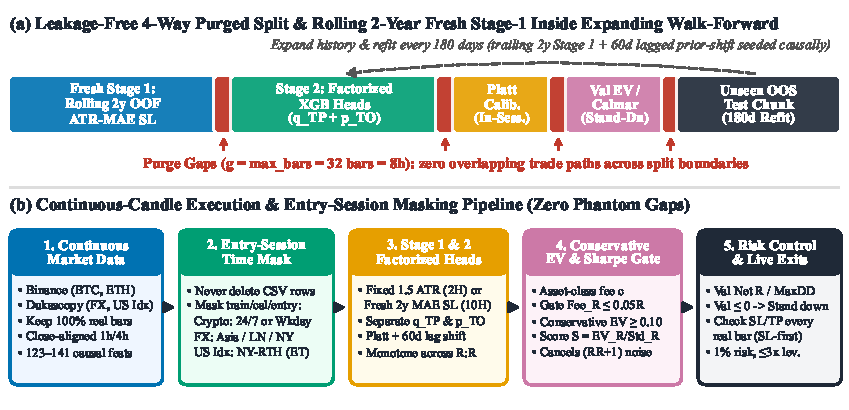
\includegraphics[width=\textwidth]{figures/fig1_pipeline_architecture.pdf}
  \caption{\textbf{End-to-end leakage-free architecture.} \textbf{(a)} Inside each $180$-day expanding walk-forward window, four time-ordered partitions are separated by $g=32$-bar purge gaps, with fresh rolling $2$-year out-of-fold Stage-1 stop models. \textbf{(b)} All features and open-trade exits run on $100\%$ continuous real candles while training, calibration, and new entries are masked to the chosen market session.}
  \label{fig:architecture}
\end{figure}

\paragraph{Causal Feature Engineering and Selection.}
We compute $123$ pure OHLCV features across all nine symbols (returns, realized volatility, ATR\%, candlestick body/wick ratios, EMA/RSI/MACD/Bollinger/ADX indicators, close-aligned $1\text{h}$/$4\text{h}$ trend features, and cyclical UTC time encodings) plus $16$--$18$ Binance order-flow and derivatives features on \texttt{BTC}/\texttt{ETH} (Spot and Perpetual taker-buy ratios, cumulative volume delta, average trade size, perp-spot basis, Premium Index, and $8\text{h}$ funding rates; full taxonomy in Appendix~\ref{app:features}). Inner-train feature selection experiments on \texttt{BTC 1h} established three clear lessons: (1) model-specific inner pruning reduced noise (\texttt{LSTM} $135 \to 19$, Logistic Regression $135 \to 30$, \texttt{XGBoost} $131 \to 55$); (2) weighting training labels by $|r_{t+1}|$ hurt OOS accuracy by $2.2$--$3.1\text{ pp}$ because volatility spikes dominated gradients; and (3) adding native Binance Perpetual order-flow features lifted \texttt{BTC 15m} 10-head test ROC-AUC from $0.609$ (OHLCV-only) to $0.662$ ($+0.054$ AUC).

% ==============================================================================
\section{Model Architectures and Training Methodology}
\label{sec:models}

\subsection{Phase 1: Three-Model Next-Candle Consensus (\texttt{BTC 1h})}

To test standard next-candle prediction cleanly, we train three different model families on identical time-ordered splits of \texttt{BTC 1h}: (1) a $5$-seed bagged regularized \texttt{XGBoost} ($55$ features, \texttt{max\_depth=4}), (2) a PyTorch \texttt{LSTM} ($19$ features, $24$-hour lookback, $32$ hidden units, \texttt{AdamW}), and (3) an L1/L2-regularized Logistic Regression ($30$ features with inner-fitted \texttt{RobustScaler}). Each model is Platt-calibrated on a purged slice, and we compare four ensemble rules: \texttt{three\_majority}, \texttt{soft\_weighted}, \texttt{meta\_stacking}, and \texttt{three\_unanimous}.

\subsection{Phase 2: Two-Stage Factorized Multi-R:R Bracket Model (\texttt{15m})}

Our Phase-2 V2.2 architecture (Algorithm~\ref{alg:multirr}) directly predicts cost-adjusted barrier probabilities in three stages, supporting both \textbf{Learned-SL 10-Head} ($\mathcal{R}=\{2.0,2.5,3.0,3.5,4.0\}$) and a simpler \textbf{Fixed-ATR 2-Head} baseline ($1.5\,\ATR$, $\mathcal{R}=\{2.5\}$).

\paragraph{Stage 1: Fresh Rolling $2$-Year ATR-Normalized Stop-Losses.}
To make stop widths dimensionless across assets with vastly different volatility scales, we compute causal $14$-bar $\ATR\%_t = \ATR_{14}(t) / C_t$ and $8$-bar Maximum Adverse Excursion targets from entry $e = O_{t+1}$:
\begin{align}
  \MAE_{8,\mathrm{long}}(t) &= \max\!\left(0,\; \frac{O_{t+1} - \min_{k=1..8} L_{t+k}}{O_{t+1}}\right), \notag \\
  \MAE_{8,\mathrm{short}}(t) &= \max\!\left(0,\; \frac{\max_{k=1..8} H_{t+k} - O_{t+1}}{O_{t+1}}\right).
  \label{eq:mae}
\end{align}
An early version of our pipeline trained Stage~1 only on the first $38\%$ of history, leaving Stage~1 stops $4$ years out of date by 2026. In V2.2, we fix this by generating $4$-fold chronological out-of-fold quantile \texttt{XGBoost} regressors ($\alpha=0.70$, trailing $2$-year window, trained on in-session bars $M_{\mathrm{sess}}(t)=1$) inside training, and fitting a fresh trailing $2$-year Stage-1 pair right before each $180$-day test chunk:
\begin{align}
  \widehat{m}_s(\mathbf{x}_t) &= \widehat{Q}_{0.70}\!\left(\frac{\MAE_{8,s}(t)}{\ATR\%_t} \;\middle|\; \mathbf{x}_t\right), \notag \\
  \hat{\delta}_s(t) &= \operatorname{clip}\!\Bigl(\operatorname{clip}\bigl(\widehat{m}_s(\mathbf{x}_t), 0.8, 3.5\bigr)\cdot \ATR\%_t,\; \max(0.0005, 5c),\; 0.030\Bigr).
  \label{eq:stage1_sl}
\end{align}
For the Fixed-ATR baseline, Eq.~\eqref{eq:stage1_sl} simplifies to $\hat{\delta}_s(t) = \operatorname{clip}(1.5\,\ATR\%_t, \max(0.0005, 5c), 0.030)$.

\paragraph{Stage 2: Chain-Rule Factorized Heads, Lagged 60-Day Recalibration, and Monotone Projection.}
For each side $s$ and ratio $r$, we factor the take-profit probability cleanly by separating direction from timeout:
\begin{equation}
  p_{\TP}^{(s,r)}(\mathbf{x}_t) \;=\; \bigl(1 - p_{\mathrm{TO}}^{(s,r)}(\mathbf{x}_t)\bigr)\cdot q_{\TP}^{(s,r)}(\mathbf{x}_t),
  \label{eq:factorized}
\end{equation}
where $q_{\TP} = \mathbb{P}(\TP \mid \TP\text{ or }\SL, \mathbf{x}_t)$ is a regularized \texttt{XGBoost} binary classifier trained only on resolved $\TP/\SL$ bars (so early stopping focuses purely on direction), and $p_{\mathrm{TO}} = \mathbb{P}(\mathrm{TIMEOUT} \mid \mathbf{x}_t)$ is a separate timeout classifier. Both heads are calibrated via Platt scaling strictly on in-session tradable bars ($\FeeR \le 0.05R$ and $M_{\mathrm{sess}}=1$). To adapt to regime shifts without lookahead, we apply a lagged $60$-day ($W = 5{,}760$ bars, lag $= H+1 = 33$ bars) rolling prior-shift adjustment in logit space:
\begin{align}
  \Delta_t &= \operatorname{clip}\!\Bigl(\logit(\bar{y}_{t-\mathrm{lag}}) - \logit(\bar{p}_{t-\mathrm{lag}}),\; -1.5,\; +1.5\Bigr), \notag \\
  \tilde{p}(t) &= \sigma\!\Bigl(\logit(p^{\mathrm{cal}}(t)) + \Delta_t\Bigr),
  \label{eq:rolling_cal}
\end{align}
applied independently to $q_{\TP}$ and $p_{\mathrm{TO}}$ on active bars, followed by gentle shrinkage ($5\%$) toward the prior and monotonic projection $\hat{p}_{s, r_j}(t) = \min(\hat{p}_{s, r_{j-1}}(t), p_{\TP}^{(s,r_j)}(t))$ so harder targets never have higher probability than easier ones.

\paragraph{Stage 3: Conservative Validation Thresholding and Automatic Stand-Down.}
On the purged validation slice, we sweep $\tau_{\mathrm{ev}} \in \{0.10, 0.14, 0.18, 0.22, 0.26, 0.30\}R$ using conservative EV (Eq.~\eqref{eq:ev_exact}), the fee gate $\FeeR \le 0.05R$, the session mask $M_{\mathrm{sess}}$, and Per-Trade Sharpe selection (Eq.~\eqref{eq:sharpe_score}), choosing $\tau^*_{\mathrm{ev}}$ to maximize validation $\mathrm{Calmar}_R = \text{Net }R / \max(\mathrm{MaxDD}_\%, 1.0)$. If \emph{every} threshold in the grid has validation $\text{Net }R \le 0$ (or fewer than $2$ trades), the model selects \texttt{STAND\_DOWN} ($\tau^*_{\mathrm{ev}} = +\infty$) and takes zero trades in the upcoming test chunk.

\begin{algorithm}[t]
\caption{Leakage-Free Continuous-Candle Walk-Forward Multi-R:R Training and Execution (V2.2)}
\label{alg:multirr}
\small
\textbf{Input:} Continuous chronological data $\mathcal{D}$; outer split $N_0 = \lfloor 0.8T \rfloor$; chunk size $K = 180\text{d}$; purge gap $g = H$; session mask $M_{\mathrm{sess}}$; fee rate $c$; ratios $\mathcal{R}$.
\begin{enumerate}
  \item \textbf{for} expanding chunk $t_{\mathrm{start}} = N_0, N_0+K, \dots < T$ \textbf{do}
  \item \quad Partition history $\mathcal{D}_{1:t_{\mathrm{start}}}$ via Eq.~\eqref{eq:purged_split} with $g$-bar purge gaps.
  \item \quad \textbf{Stage 1:} Fit $4$-fold rolling $2$-year OOF quantile SL models on $M_{\mathrm{sess}}=1$ bars (or use Fixed $1.5\,\ATR$), plus a fresh trailing $2$-year Stage-1 model for the unseen test chunk.
  \item \quad \textbf{Stage 2:} Compute 3-class barrier labels on $100\%$ continuous bars; train factorized $q_{\TP}$ and $p_{\mathrm{TO}}$ heads on $M_{\mathrm{sess}}=1$ bars; Platt-calibrate on tradable ($\FeeR \le 0.05R, M_{\mathrm{sess}}=1$) bars.
  \item \quad \textbf{Stage 3:} Run causal $60$d lagged shift (Eq.~\eqref{eq:rolling_cal}) and monotone projection on validation; pick $\tau^*_{\mathrm{ev}} = \arg\max \mathrm{Calmar}_R$ under conservative EV; if best validation $\text{Net }R \le 0$, set \texttt{STAND\_DOWN}.
  \item \quad Simulate unseen chunk $\mathcal{T}$: check SL/TP/timeout on \emph{every} continuous bar; allow new entries only when $M_{\mathrm{sess}}=1$, $\FeeR \le 0.05R$, and $\EVR^{\mathrm{cons}} > \tau^*_{\mathrm{ev}}$ via Sharpe score $S$.
  \item \textbf{end for}
\end{enumerate}
\end{algorithm}

% ==============================================================================
\section{Experimental Results}
\label{sec:results}

\subsection{Phase 1: Why Next-Candle Prediction Fails (\texttt{BTC 1h})}
\label{sec:phase1_results}

Table~\ref{tab:phase1} and Figure~\ref{fig:phase1} show our Phase-1 results on $59{,}904$ hourly Bitcoin candles:
\begin{itemize}
    \item \textbf{Real but Small Signal:} On the $11{,}979$-hour holdout (majority class $49.97\%$), all three individual models beat chance ($52.72\%$--$53.13\%$). Combining them raises accuracy (\texttt{three\_majority} $53.41\%$, \texttt{three\_unanimous} $53.73\%$ at $72.2\%$ coverage; block-bootstrap $95\%$ CI $[52.29\%, 54.10\%]$, $p < 0.001$) and yields tight calibration (\texttt{meta\_stacking} $\mathrm{ECE} = 0.0086$).
    \item \textbf{Accuracy Drops Over Time:} Across the $3$-fold walk-forward ($44{,}911$ hours, Figure~\ref{fig:phase1}a), unanimous accuracy falls steadily from $57.99\%$ ($2021$--$2023$) to $56.21\%$ ($2023$--$2025$) and $54.29\%$ ($2025$--$2026$), showing that Bitcoin has become harder to predict over time~\citep{Bustos2025}.
    \item \textbf{Zero Tradable Brackets:} Even though confidence filtering reaches $59.05\%$ accuracy at $8.9\%$ coverage (Figure~\ref{fig:phase1}b), passing those well-calibrated $1$-hour probabilities into an exact fee-adjusted EV backtest over $24$--$48$h brackets rejects \emph{all $11{,}979 / 11{,}979$ hours} ($0$ trades). Predicting the next candle is simply the wrong objective for multi-hour bracket trading.
\end{itemize}

\begin{table}[t]
  \centering
  \caption{\textbf{Phase-1 \texttt{BTC 1h} next-candle directional benchmark ($59{,}904$ bars, $2020$--$2026$).} Left: $3$-fold walk-forward ($44{,}911$ OOS hours). Right: $11{,}979$-hour holdout (majority baseline $49.97\%$; $p<0.001$).}
  \label{tab:phase1}
  \scriptsize
  \setlength{\tabcolsep}{3.5pt}
  \begin{tabular}{@{}lcccc|cccc@{}}
    \toprule
    & \multicolumn{4}{c|}{\textbf{3-Fold Walk-Forward Acc.\ (\%)}} & \multicolumn{4}{c}{\textbf{Holdout ($n=11{,}979$ OOS hrs)}} \\
    Model / Ensemble & Fold 1 & Fold 2 & Fold 3 & Mean & Acc.\ (\%) & ROC-AUC & ECE / LL & Cov. \\
    \midrule
    XGBoost (55 feats, 5-seed) & 54.66 & 54.70 & 52.80 & 54.05 & 52.94 & \textbf{0.5461} & LL 0.6906 & 100.0\% \\
    LSTM (19 feats, $\mathrm{lb}=24$) & 54.85 & 54.96 & 52.76 & 54.19 & 52.72 & 0.5415 & LL 0.6909 & 100.0\% \\
    Logistic Reg.\ (30 feats, 2y) & 54.80 & 55.00 & 53.51 & 54.44 & 53.13 & 0.5420 & LL 0.6928 & 100.0\% \\
    \midrule
    \texttt{three\_majority} & 55.53 & 55.18 & 53.18 & 54.63 & \textbf{53.41} & --- & --- & 100.0\% \\
    \texttt{soft\_weighted} & 54.76 & 55.29 & 53.32 & 54.46 & 53.30 & 0.5434 & ECE 0.0160 & 100.0\% \\
    \texttt{meta\_stacking} & 55.33 & 55.16 & 52.96 & 54.48 & 52.97 & 0.5447 & \textbf{ECE 0.0086} & 100.0\% \\
    \texttt{three\_unanimous} & \textbf{57.99} & \textbf{56.21} & \textbf{54.29} & \textbf{56.16} & 53.73 & --- & --- & 72.2\% \\
    \midrule
    \texttt{soft\_weighted} ($\mathrm{conf}\ge 0.55$) & --- & --- & --- & --- & 54.81 & --- & --- & 42.4\% \\
    \texttt{soft\_weighted} ($\mathrm{conf}\ge 0.60$) & --- & --- & --- & --- & \textbf{59.05} & --- & --- & 8.9\% \\
    \bottomrule
  \end{tabular}
\end{table}

\begin{figure}[t]
  \centering
  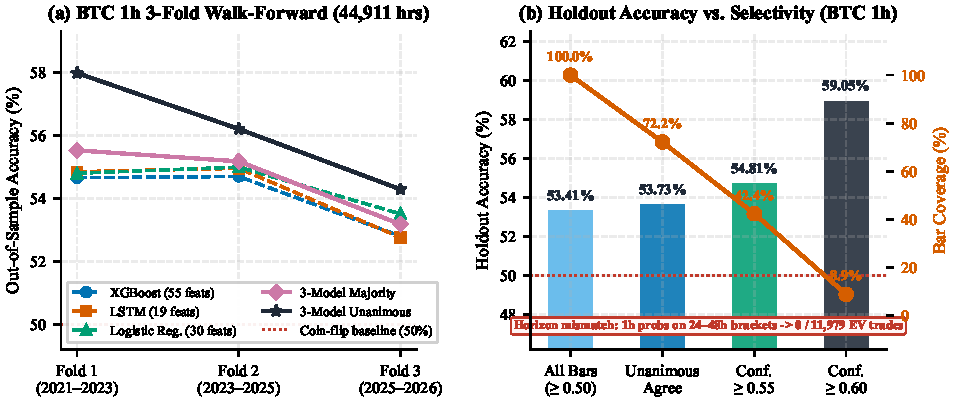
\includegraphics[width=\textwidth]{figures/fig3_consensus_1h_diagnostics.pdf}
  \caption{\textbf{Phase-1 \texttt{BTC 1h} directional results.} \textbf{(a)} Ensembles beat single models, but accuracy declines steadily from Fold~1 to Fold~3 as the market matures. \textbf{(b)} High-confidence bars reach $59.05\%$ accuracy, yet mapping $1$-hour probabilities to $24$--$48$h brackets passes $0 / 11{,}979$ EV checks.}
  \label{fig:phase1}
\end{figure}

\subsection{Phase 2: Payoff Audit and Architecture Comparison on \texttt{BTC} and \texttt{ETH}}
\label{sec:audit}

Before testing across asset classes and time zones, we conducted a controlled audit on $24/7$ \texttt{BTC} and \texttt{ETH} ($47{,}924$ OOS $15\text{m}$ bars each, June 2025--October 2026) to isolate the exact effect of timeout payoff modeling, fresh Stage-1 stops, and model complexity (Table~\ref{tab:btc_eth_audit} and Figure~\ref{fig:v2_audit}a):

\begin{enumerate}
    \item \textbf{Crediting Timeouts in the Entry Gate Fails:} We tested three exact-timeout implementations of Eq.~\eqref{eq:ev_3outcome}: \textbf{V2} (joint 3-class XGBoost), \textbf{V2.1} (factorized 3-outcome EV using $q_{\TP}, p_{\mathrm{TO}}, \widehat{\mu}_{\mathrm{TO}}(\mathbf{x}_t)$), and \textbf{V3} (direct regression on realized simulator Net $R$). Even though V2.1 predicted conditional timeout payoff accurately ($+0.84R$ predicted vs.\ $+0.84R$ realized on \texttt{BTC}), all three timeout-crediting gates overtraded heavily ($157$--$1{,}102$ trades) and lost money (\texttt{BTC} $-4.67R$ to $-89.68R$; \texttt{ETH} $-22.08R$ to $-33.42R$, or $+19.82R$ with $29.9\%$ DD). Because timeout timing ($\mathrm{to\_AUC} = 0.69$--$0.74$) is far easier to predict than price direction ($\mathrm{dir\_AUC} = 0.55$--$0.59$), giving credit for timeouts floods the strategy with slow, low-edge entries.
    \item \textbf{Fresh Rolling 2-Year Stage-1 + Conservative Gate Works:} Keeping the clean factorized probabilities $p_{\TP} = (1 - p_{\mathrm{TO}}) q_{\TP}$ inside the \emph{conservative} entry gate (\textbf{V2.2 Fresh-S1 10H}) and refreshing Stage-1 stops on a trailing $2$-year window tripled \texttt{BTC} profit from $+1.29R$ (stale Stage~1) to $\mathbf{+4.25R}$ ($\PF = 1.19$, MaxDD halved to $\mathbf{3.57\%}$, \texttt{ExpEV} $+0.201R$ vs.\ \texttt{RealR} $+0.125R$), while \texttt{ETH} earned $+5.29R$ ($\PF = 1.05$) for a combined $\mathbf{+9.54R}$.
    \item \textbf{Simpler 2-Head Fixed-ATR Removes Selection Noise on \texttt{ETH}:} Comparing the $10$-head Learned-SL model against a simpler $2$-head (\texttt{Long}/\texttt{Short}) \textbf{Fixed-ATR ($1.5\,\ATR$), Single-$\RR$ ($2.5{:}1$)} baseline showed that \texttt{ETH} jumped to $\mathbf{+17.23R}$ ($+15.65\%$, $\PF = 1.12$, $168$ trades) with tight selected-trade calibration (\texttt{ExpEV} $+0.138R$ vs.\ \texttt{RealR} $+0.103R$, gap $0.035R$ vs.\ $0.112R$ for $10$ heads) and balanced profit across both $30$-day bull ($+8.57R$) and bear ($+8.66R$) markets. On \texttt{BTC}, Fixed-ATR stood down safely ($0.00R$, $0.00\%$ DD), showing that learned stops specifically helped \texttt{BTC} ($+4.25R$).
\end{enumerate}

\begin{table}[t]
  \centering
  \caption{\textbf{Controlled payoff and architecture audit on continuous 24/7 \texttt{BTC} and \texttt{ETH} ($15\text{m}$ OOS, $c=1.0\text{ bp}$/side, $\FeeR \le 0.05R$).} Top: crediting timeouts (V2, V2.1, V3) degrades trade selection. Bottom: conservative lower-bound gating (V2.2) succeeds with both Fresh-S1 10-Head and Fixed-ATR 2-Head.}
  \label{tab:btc_eth_audit}
  \scriptsize
  \setlength{\tabcolsep}{3.0pt}
  \begin{tabular}{@{}llrrrrrrrr@{}}
    \toprule
    Asset \& Variant & Stop / Heads / EV Gate & Tr. & WR\% & PF & Net $R$ & DD\% & Exp/Real $R$ & BalAcc & AUC \\
    \midrule
    \texttt{BTC} V2 Joint 3-Class & Fresh S1 / 10H / 3-Out & 324 & 34.6 & 0.91 & $-15.27$ & 19.87 & $+.234/-.047$ & 50.81\% & .609 \\
    \texttt{BTC} V2.1 Fact.\ 3-Out & Fresh S1 / 10H / 3-Out & 157 & 37.6 & 0.93 & $-4.67$ & 14.58 & $+.309/-.030$ & 50.24\% & .594 \\
    \texttt{BTC} V3 Direct Net-$R$ & Fresh S1 / 10H / Direct & 1102 & 33.4 & 0.86 & $-89.68$ & 64.37 & $+.130/-.081$ & IC $-.002$ & --- \\
    \texttt{ETH} V2 Joint 3-Class & Fresh S1 / 10H / 3-Out & 587 & 34.9 & 1.03 & $+19.82$ & 29.90 & $+.287/+.034$ & 51.28\% & .607 \\
    \texttt{ETH} V2.1 Fact.\ 3-Out & Fresh S1 / 10H / 3-Out & 811 & 34.7 & 0.94 & $-33.42$ & 54.90 & $+.236/-.041$ & 50.49\% & .598 \\
    \texttt{ETH} V3 Direct Net-$R$ & Fresh S1 / 10H / Direct & 507 & 33.9 & 0.93 & $-22.08$ & 38.33 & $+.180/-.044$ & IC $+.010$ & --- \\
    \midrule
    \texttt{BTC} V1 Stale-S1 10H & First-38\% / 10H / Cons. & 31 & 29.0 & 1.04 & $+1.29$ & 6.54 & $+.222/+.041$ & 50.73\% & .600 \\
    \texttt{BTC} \textbf{V2.2 Fresh 10H} & Fresh S1 / 10H / Cons. & 34 & 35.3 & \textbf{1.19} & $\mathbf{+4.25}$ & \textbf{3.57} & $+.201/+.125$ & 50.34\% & .598 \\
    \texttt{ETH} \textbf{V2.2 Fresh 10H} & Fresh S1 / 10H / Cons. & 119 & 32.8 & 1.05 & $+5.29$ & 13.44 & $+.156/+.044$ & 50.70\% & .600 \\
    \texttt{BTC} V2.2 Fixed-ATR 2H & $1.5\,\ATR$ / 2.5:1 / Cons. & 0 & --- & --- & $0.00$ & \textbf{0.00} & \textsc{StandDown} & 50.67\% & .573 \\
    \texttt{ETH} \textbf{V2.2 Fixed-ATR 2H} & $1.5\,\ATR$ / 2.5:1 / Cons. & 168 & 33.3 & \textbf{1.12} & $\mathbf{+17.23}$ & 16.55 & $\mathbf{+.138/+.103}$ & 51.55\% & .576 \\
    \bottomrule
  \end{tabular}
\end{table}

\begin{figure}[t]
  \centering
  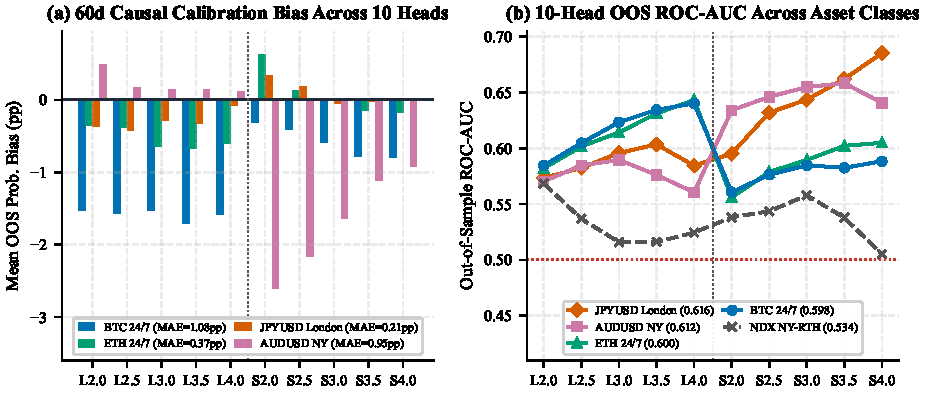
\includegraphics[width=\textwidth]{figures/fig4_calibration_and_auc.pdf}
  \caption{\textbf{OOS probability calibration and 10-head ROC-AUC across asset classes (real saved logs).} \textbf{(a)} After lagged $60$-day prior-shift recalibration, mean probability bias across all $10$ heads stays low across \texttt{BTC}, \texttt{ETH}, \texttt{JPYUSD} (London), and \texttt{AUDUSD} (New York). \textbf{(b)} OOS ROC-AUC climbs steadily with $\RR$ across crypto and active-session Forex heads, while \texttt{NDX} NY-RTH remains weaker on pure OHLCV.}
  \label{fig:cal_auc}
\end{figure}

\begin{figure}[t]
  \centering
  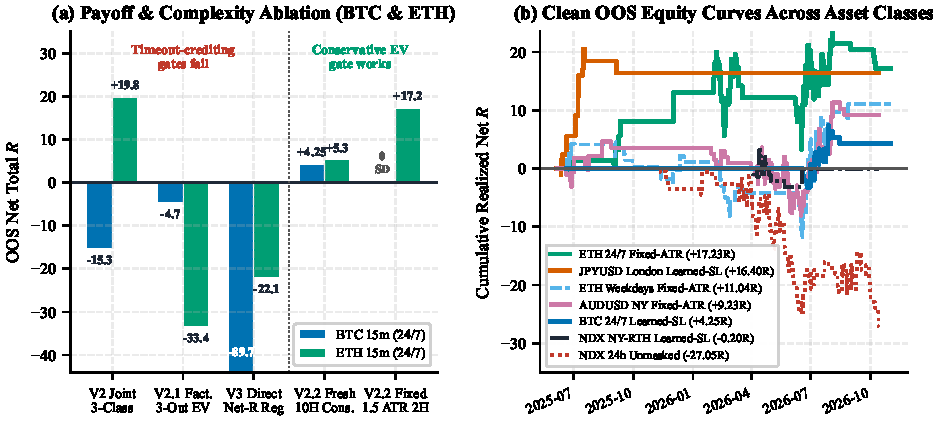
\includegraphics[width=\textwidth]{figures/fig5_v2_payoff_and_equity.pdf}
  \caption{\textbf{Payoff ablation and clean OOS equity curves.} \textbf{(a)} Crediting timeout payoffs inside the entry gate fails on \texttt{BTC} and \texttt{ETH}, whereas conservative EV succeeds on both Fixed-ATR and Fresh-S1 10-Head. \textbf{(b)} Step-by-step realized Net $R$ curves from saved logs across crypto, Forex, and US equity indices (showing how NY-RTH masking eliminates the $-27.05R$ \texttt{NDX} 24h loss).}
  \label{fig:v2_audit}
\end{figure}

\subsection{How Market Time Zones Control Profitability Across All Nine Symbols}
\label{sec:timezone_results}

A major finding of our cross-asset study is that \textbf{an accurate signal is not enough on its own: the market time zone strongly determines whether the strategy makes or loses money}. Using our clean continuous-candle entry-session masking (\texttt{--entry-session}, zero phantom gaps), we evaluated every Forex pair across five trading windows, \texttt{BTC}/\texttt{ETH} across 24/7 vs.\ weekdays-only, and \texttt{SPX}/\texttt{NDX} across full 24h vs.\ New York Regular Trading Hours (Tables~\ref{tab:fx_timezones}--\ref{tab:cross_asset_sessions} and Figure~\ref{fig:timezone}).

\subsubsection{G10 Forex Time Zone Analysis (5 Pairs \texorpdfstring{$\times$}{x} 5 Sessions)}

Table~\ref{tab:fx_timezones} reveals a striking pattern across all five \texttt{XXX-USD} Forex pairs:
\begin{itemize}
    \item \textbf{Asian Session ($00{:}00$--$09{:}00$ UTC) Is Pure Noise:} Mean OOS ROC-AUC drops to $\mathbf{0.513}$ on both Fixed-ATR and Learned-SL (indistinguishable from a coin flip). Fixed-ATR loses $\mathbf{-42.28R}$ across $152$ trades (\texttt{EURUSD} $-23.38R$, \texttt{AUDUSD} $-22.13R$), while Learned-SL stands down or loses slightly ($-0.40R$). Even though Sydney and Tokyo are open, \texttt{XXX-USD} pairs lack institutional USD order flow during these hours and have much wider intraday volatility swings ($2.1\times$--$2.5\times$).
    \item \textbf{New York Session ($12{:}00$--$21{:}00$ UTC) Dominates Fixed-ATR:} Masking entries to New York hours (which includes the $12{:}00$--$16{:}00$ UTC London--New York overlap and major US macro releases) lifts OOS ROC-AUC on \emph{every single one of the five pairs}: \texttt{CADUSD} ($0.675$), \texttt{GBPUSD} ($0.666$), \texttt{EURUSD} ($0.643$), \texttt{AUDUSD} ($0.634$), and \texttt{JPYUSD} ($0.595$), raising mean AUC by $+0.130$ over Asia ($0.513 \to \mathbf{0.643}$). Total 5-pair Net $R$ swings by $\mathbf{+58.77R}$, from $-42.28R$ (Asia) to $\mathbf{+16.49R}$ with \textbf{zero losing pairs} (\texttt{AUDUSD} $+9.23R$, \texttt{JPYUSD} $+6.05R$ at $\PF=1.83$, \texttt{GBPUSD} $+1.21R$, and clean $0.00R$ stand-downs on \texttt{EURUSD} and \texttt{CADUSD}).
    \item \textbf{London Session ($07{:}00$--$16{:}00$ UTC) Dominates Learned-SL:} Under Learned-SL 10-Head, London produces the best 5-pair total at $\mathbf{+18.32R}$ with \textbf{zero losing pairs} ($\mathrm{AUC} = 0.606$), driven by \texttt{JPYUSD} ($\mathbf{+16.40R}$, $16$ trades, $\PF = 2.95$, $1.84\%$ MaxDD; see execution zoom in Figure~\ref{fig:exec_zoom}b) and \texttt{CADUSD} ($+1.92R$, $\PF = 2.10$), while \texttt{EURUSD}, \texttt{GBPUSD}, and \texttt{AUDUSD} stand down safely at $0.00\%$ drawdown. New York Learned-SL is also strongly positive ($\mathbf{+6.38R}$: \texttt{AUDUSD} $+4.28R$ at $\PF=2.84$, \texttt{JPYUSD} $+4.18R$ at $\PF=5.01$), and London+NY reaches the highest Learned-SL mean AUC ($0.625$, $+3.01R$, with \texttt{JPYUSD} $+15.23R$ at $\PF=1.66$).
    \item \textbf{Weekdays 24h Fails Because It Mixes Asian Noise with Active Hours:} Running all 24 weekday hours on Fixed-ATR loses $-19.57R$ (\texttt{EURUSD} $-19.82R$) because quiet Asian entries contaminate training and calibration. Removing Asia immediately turns the basket positive ($+10.79R$ in London+NY, $+16.49R$ in New York).
\end{itemize}

\begin{table}[t]
  \centering
  \caption{\textbf{G10 Forex time zone comparison across all five pairs ($15\text{m}$ OOS, $100\%$ continuous real candles, $c=0.2\text{ bp}$/side, $H=32$).} Every cell reports realized OOS Net $R$ and mean OOS ROC-AUC in parentheses. Asia behaves like coin-flip noise ($\mathrm{AUC}=0.513$), while New York (Fixed-ATR) and London (Learned-SL) produce $+16.49R$ and $+18.32R$ with zero losing pairs.}
  \label{tab:fx_timezones}
  \scriptsize
  \setlength{\tabcolsep}{3.0pt}
  \begin{tabular}{@{}llrrrrr@{}}
    \toprule
    Arch. & Symbol & Asia ($00$--$09$) & London ($07$--$16$) & New York ($12$--$21$) & LN+NY ($07$--$21$) & Weekdays 24h \\
    \midrule
    \multirow{6}{*}{\shortstack[l]{\textbf{Fixed-ATR}\\\textbf{2-Head}\\($1.5\,\ATR$,\\$2.5{:}1$)}}
    & \texttt{EURUSD} & $-23.38R$ (.490) & $0.00R$ (.573) & $\mathbf{0.00R}$ (\textbf{.643}) & $-3.14R$ (.640) & $-19.82R$ (.604) \\
    & \texttt{GBPUSD} & $0.00R$ (.506) & $\mathbf{+3.85R}$ (.570) & $\mathbf{+1.21R}$ (\textbf{.666}) & $+2.46R$ (.651) & $0.00R$ (.622) \\
    & \texttt{JPYUSD} & $+3.23R$ (.511) & $+2.56R$ (.587) & $\mathbf{+6.05R}$ (\textbf{.595}) & $+4.17R$ (.579) & $0.00R$ (.569) \\
    & \texttt{AUDUSD} & $-22.13R$ (.517) & $-2.85R$ (.553) & $\mathbf{+9.23R}$ (\textbf{.634}) & $+9.33R$ (.610) & $+0.25R$ (.578) \\
    & \texttt{CADUSD} & $0.00R$ (.542) & $0.00R$ (.565) & $\mathbf{0.00R}$ (\textbf{.675}) & $-2.03R$ (.663) & $0.00R$ (.621) \\
    \cmidrule(lr){2-7}
    & \textbf{5-FX Total / Mean} & $\mathbf{-42.28R}$ (.513) & $\mathbf{+3.56R}$ (.570) & $\mathbf{+16.49R}$ (\textbf{.643}) & $\mathbf{+10.79R}$ (.629) & $\mathbf{-19.57R}$ (.599) \\
    \midrule
    \multirow{6}{*}{\shortstack[l]{\textbf{Learned-SL}\\\textbf{10-Head}\\(Fresh 2y,\\$2.0$--$4.0$)}}
    & \texttt{EURUSD} & $+0.87R$ (.501) & $0.00R$ (.608) & $0.00R$ (.603) & $-4.60R$ (.618) & --- \\
    & \texttt{GBPUSD} & $+0.07R$ (.501) & $0.00R$ (.597) & $0.00R$ (.582) & $0.00R$ (.627) & --- \\
    & \texttt{JPYUSD} & $0.00R$ (.547) & $\mathbf{+16.40R}$ (\textbf{.616}) & $+4.18R$ (.608) & $+15.23R$ (.600) & --- \\
    & \texttt{AUDUSD} & $0.00R$ (.494) & $0.00R$ (.595) & $\mathbf{+4.28R}$ (.612) & $-7.62R$ (.612) & --- \\
    & \texttt{CADUSD} & $-1.34R$ (.527) & $\mathbf{+1.92R}$ (.615) & $-2.08R$ (.560) & $0.00R$ (\textbf{.671}) & --- \\
    \cmidrule(lr){2-7}
    & \textbf{5-FX Total / Mean} & $\mathbf{-0.40R}$ (.514) & $\mathbf{+18.32R}$ (.606) & $\mathbf{+6.38R}$ (.593) & $\mathbf{+3.01R}$ (\textbf{.625}) & --- \\
    \bottomrule
  \end{tabular}
\end{table}

\subsubsection{Crypto (24/7 vs.\ Weekdays) and US Equity Indices (24h vs.\ New York RTH)}

Table~\ref{tab:cross_asset_sessions} and Figure~\ref{fig:timezone}(b) summarize the time-zone behavior of \texttt{BTC}, \texttt{ETH}, \texttt{SPX}, and \texttt{NDX} alongside the row-deletion artifact check:

\begin{itemize}
    \item \textbf{Crypto (\texttt{BTC}, \texttt{ETH}) — Full 24/7 vs.\ Weekdays-Only:} When we first tested dropping weekends by deleting Saturday/Sunday rows from the CSV, \texttt{BTC} fell to $-14.49R$ and \texttt{ETH} collapsed to $-32.66R$ ($-47.15R$ total). That drop looked puzzling at first, but our audit proved it was caused by fake $48$-hour weekend gaps corrupting Monday indicators. Switching to \emph{clean continuous-candle weekday masking} immediately fixed \texttt{ETH} Fixed-ATR to $\mathbf{+11.04R}$ ($127$ trades, $\PF = 1.11$, $+9.44\%$) and \texttt{BTC} Learned-SL to $0.00R$ stand-down ($0.00\%$ DD). Even with clean masking, however, full 24/7 trading remains better (\texttt{ETH} $+17.23R$ Fixed-ATR; \texttt{BTC} $+4.25R$ and \texttt{ETH} $+5.29R$ Learned-SL) because crypto markets trade continuously and blocking weekends discards $28.6\%$ of training and calibration data without protecting Friday positions from weekend moves.
    \item \textbf{US Equity Indices (\texttt{SPX}, \texttt{NDX}) — 24h Overnight Trap vs.\ New York RTH:} On unmasked 24-hour index data, intraday volatility jumps $\mathbf{3.8\times}$ from overnight Globex ($05{:}00$ UTC, median $\ATR = 0.074\%$) to the US cash open ($15{:}00$--$17{:}00$ UTC, $0.283\%$). Because $32$ bars ($8$ hours) after $05{:}00$ UTC always lands on the $09{:}30$ AM ET opening bell, Stage-1 Learned-SL inflates overnight stops above the $0.20\%$ fee floor while Stage~2 sees low timeout rates ahead of the bell—dumping $\mathbf{154 / 157}$ ($98.1\%$) of \texttt{NDX} trades into dead overnight hours and losing $\mathbf{-27.05R}$ ($-15.16R$ on Fixed-ATR). Restricting entries strictly to \textbf{New York Regular Trading Hours ($09{:}30$--$16{:}00$ ET)} on continuous real candles eliminates that overnight trap completely: \texttt{SPX} stands down cleanly ($0.00R$, $0.00\%$ DD across all four configs, $\mathrm{AUC} = 0.609$), and \texttt{NDX} improves from $-27.05R$ to $0.00R$ ($H=16$) and $-0.20R$ ($H=32$, $\PF = 0.97$). At the same time, honest continuous-candle execution shows that pure OHLCV US equity indices are highly efficient during cash hours—without the fake overnight gap fills from row deletion, conservative validation rightly avoids forcing low-edge trades.
\end{itemize}

\begin{table}[t]
  \centering
  \caption{\textbf{Cross-asset session comparison for Crypto (\texttt{BTC}, \texttt{ETH}) and US Equity Indices (\texttt{SPX}, \texttt{NDX}).} All primary rows use $100\%$ continuous real candles with entry-only session masking. The bottom two rows show naive CSV row deletion for contrast, proving how row deletion creates fake losses on crypto and fake gap profits on \texttt{SPX}.}
  \label{tab:cross_asset_sessions}
  \scriptsize
  \setlength{\tabcolsep}{3.1pt}
  \begin{tabular}{@{}lllrrrrrrr@{}}
    \toprule
    Symbol & Session Mode & Arch.\ ($H$) & Tr. & WR\% & PF & Net $R$ & Ret\% & DD\% & AUC \\
    \midrule
    \texttt{BTC} & Continuous 24/7 & Learned 10H (32) & 34 & 35.3 & \textbf{1.19} & $\mathbf{+4.25}$ & +3.44 & \textbf{3.57} & .598 \\
    \texttt{ETH} & Continuous 24/7 & Fixed 2H (32) & 168 & 33.3 & \textbf{1.12} & $\mathbf{+17.23}$ & +15.65 & 16.55 & .576 \\
    \texttt{ETH} & Continuous 24/7 & Learned 10H (32) & 119 & 32.8 & 1.05 & $+5.29$ & +4.28 & 13.44 & .600 \\
    \texttt{BTC} & Entry-Mask Weekdays & Learned 10H (32) & 0 & --- & --- & $0.00$ & 0.00 & \textbf{0.00} & .607 \\
    \texttt{BTC} & Entry-Mask Weekdays & Fixed 2H (32) & 21 & 23.8 & 0.73 & $-4.36$ & $-4.30$ & 8.65 & .586 \\
    \texttt{ETH} & Entry-Mask Weekdays & Fixed 2H (32) & 127 & 33.9 & \textbf{1.11} & $\mathbf{+11.04}$ & +9.44 & 16.63 & .591 \\
    \texttt{ETH} & Entry-Mask Weekdays & Learned 10H (32) & 195 & 33.3 & 0.95 & $-4.52$ & $-6.21$ & 18.32 & .614 \\
    \midrule
    \texttt{NDX} & Continuous 24h (Unmasked) & Learned 10H (32) & 157 & 26.8 & 0.77 & $-27.05$ & $-17.89$ & 19.79 & .627 \\
    \texttt{NDX} & Continuous 24h (Unmasked) & Fixed 2H (32) & 107 & 26.2 & 0.81 & $-15.16$ & $-10.68$ & 19.06 & .610 \\
    \texttt{SPX} & Continuous 24h (Unmasked) & Fixed 2H (32) & 9 & 33.3 & 0.89 & $-0.26$ & $-0.54$ & 4.16 & .616 \\
    \texttt{NDX} & Entry-Mask NY-RTH (ET) & Learned 10H (32) & 17 & 29.4 & 0.97 & $\mathbf{-0.20}$ & $-0.40$ & 6.33 & .534 \\
    \texttt{NDX} & Entry-Mask NY-RTH (ET) & Fixed 2H (16) & 0 & --- & --- & $\mathbf{0.00}$ & 0.00 & \textbf{0.00} & .608 \\
    \texttt{SPX} & Entry-Mask NY-RTH (ET) & Fixed 2H (16/32) & 0 & --- & --- & $\mathbf{0.00}$ & 0.00 & \textbf{0.00} & .609 \\
    \midrule
    \texttt{ETH} & \emph{Flawed Row-Del.\ Weekdays*} & Learned 10H (32) & 97 & 23.7 & 0.58 & $-32.66^*$ & $-27.72^*$ & $31.21^*$ & .589 \\
    \texttt{SPX} & \emph{Flawed Row-Del.\ NY-RTH*} & Fixed 2H (16) & 20 & 50.0 & 1.85 & $+10.52^*$ & $+7.53^*$ & $4.53^*$ & .636 \\
    \bottomrule
  \end{tabular}
\end{table}

\begin{figure}[t]
  \centering
  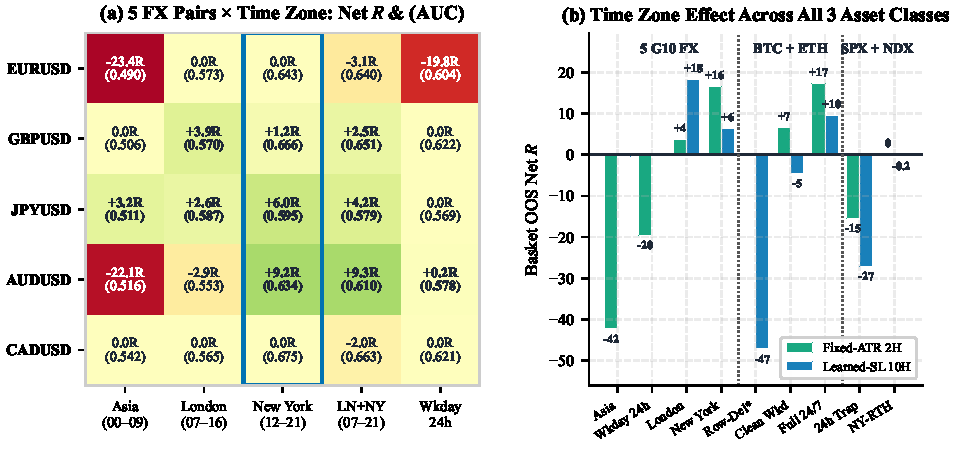
\includegraphics[width=\textwidth]{figures/fig6_timezone_profit_impact.pdf}
  \caption{\textbf{Impact of market time zones on strategy profit across all three asset classes (100\% continuous real candles).} \textbf{(a)} Heatmap of OOS Net $R$ and (AUC) across all five G10 Forex pairs and five trading sessions (Fixed-ATR 2H): Asia behaves like noise ($\mathrm{AUC}=0.513$, $-42.28R$), while New York achieves the highest AUC on every pair ($0.643$) and $+16.49R$ with zero losers. \textbf{(b)} Basket Net $R$ comparison across FX sessions, Crypto (showing the $-47.15R$ row-deletion bug vs.\ clean weekday masking and 24/7), and US equity indices (24h overnight trap vs.\ clean NY-RTH).}
  \label{fig:timezone}
\end{figure}

\begin{figure}[t]
  \centering
  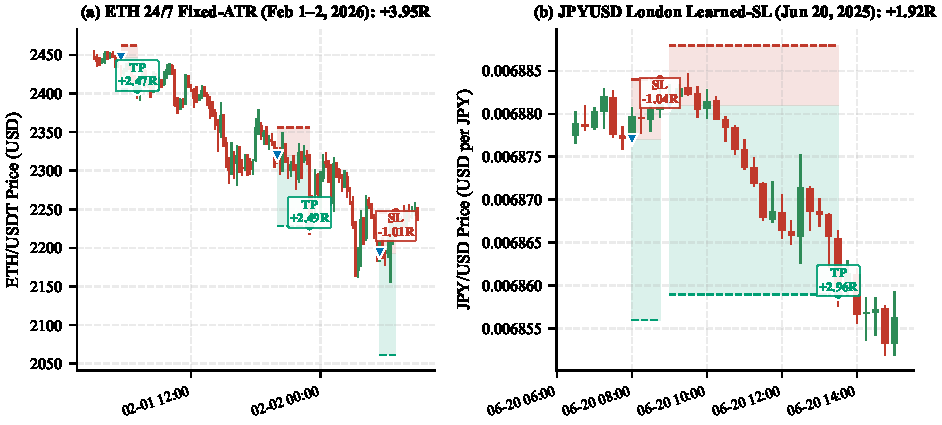
\includegraphics[width=\textwidth]{figures/fig7_trade_execution_zoom.pdf}
  \caption{\textbf{Real OOS $15\text{m}$ execution examples from saved trade logs.} \textbf{(a)} \texttt{ETH} 24/7 Fixed-ATR ($2.5{:}1$, Feb 1--2, 2026): two clean short take-profits ($+2.47R, +2.49R$) and one stop-out ($-1.01R$), netting $+3.95R$. \textbf{(b)} \texttt{JPYUSD} London Learned-SL (Jun 20, 2025): a controlled $-1.04R$ stop-out followed by a $3.0{:}1$ short breakdown ($+2.96R$) into the London--NY overlap, netting $+1.92R$. Shaded zones show exact $\SL$ and $\TP$ levels.}
  \label{fig:exec_zoom}
\end{figure}

% ==============================================================================
\section{Honest Discussion, Limitations, and Future Work}
\label{sec:discussion}

We interpret our results carefully and note four practical limits:

\begin{enumerate}
    \item \textbf{High Classification Accuracy Can Mislead:} On $10$-head models, raw classification accuracy averages $83\%$--$86\%$, yet simply predicting ``never hits $\TP$'' ($0$) scores $84\%$--$87\%$, and mean balanced accuracy sits near $50.3\%$--$52.8\%$. Headline accuracy reflects class imbalance, not trading skill; real evaluation must track selected-trade expected vs.\ realized $R$, profit factor, and drawdown.
    \item \textbf{Small Sample Sizes in Selective Sessions:} While our best session-matched runs look strong (\texttt{ETH} 24/7 Fixed-ATR $+17.23R$ over $168$ trades; \texttt{JPYUSD} London Learned-SL $+16.40R$ over $16$ trades, $\PF = 2.95$; \texttt{AUDUSD} NY Fixed-ATR $+9.23R$ over $93$ trades), several Forex and index cells fire only $1$--$17$ trades over $16$ months. Larger multi-year test spans and live paper trading are needed before claiming stable standalone alpha on low-trade pairs.
    \item \textbf{Order-Flow Features Matter:} Comparing \texttt{BTC}/\texttt{ETH} ($139$--$141$ features including taker order flow, perp-spot basis, and funding) against pure-OHLCV US equity indices (\texttt{SPX}, \texttt{NDX} standing down at $0.00R$ in NY-RTH) supports \citet{Bustos2025}: pure price indicators alone rarely overcome highly efficient cash equity markets, whereas microstructure order flow provides stronger signal.
    \item \textbf{Execution Friction Beyond Fees:} Our simulator charges realistic institutional commissions ($1.0\text{ bp}$ crypto, $0.5\text{ bp}$ US index E-mini, $0.2\text{ bp}$ FX ECN) and uses conservative stop-first tie-breaking, but does not model live order-book slippage during news spikes, spread widening, or perpetual funding cash flows while holding open crypto positions. Under higher retail fees ($4$--$5\text{ bp}$), the $\FeeR \le 0.05R$ filter would require much wider stops and sharply reduce intraday trade count.
\end{enumerate}

\paragraph{Future Work.}
Three clear next steps follow from our findings: (1) adding real CME Level-1 order-book and volume-delta features to \texttt{SPX} and \texttt{NDX} during NY-RTH to match our crypto feature richness; (2) gating Long and Short validation thresholds separately on equity indices so strong long-side trends are not cancelled by losing counter-trend shorts; and (3) combining uncorrelated crypto (24/7) and active-session Forex (London/NY) sleeves inside a single risk-budgeted portfolio tested prospectively on post-October 2026 live data.

% ==============================================================================
\section{Conclusion}
\label{sec:conclusion}

We studied why next-candle prediction fails to produce reliable trading profits and built a clean, leakage-free multi-$\RR$ expected-value pipeline tested across nine symbols in three asset classes (\texttt{BTC}, \texttt{ETH}, five G10 Forex pairs, \texttt{SPX}, and \texttt{NDX}). Our experiments establish four practical conclusions: (1) genuine $1$-hour directional signals ($53.41\%$--$59.05\%$ accuracy) fail when applied to mismatched multi-hour brackets ($0 / 11{,}979$ EV trades); (2) gating entries on a conservative lower-bound expected value prevents easily predicted timeouts from flooding execution with low-edge trades, lifting \texttt{BTC} 24/7 to $+4.25R$ ($\PF=1.19$, $3.57\%$ DD) and \texttt{ETH} 24/7 Fixed-ATR to $+17.23R$ ($\PF=1.12$, equally balanced across bull and bear markets); (3) \textbf{market time zone strongly controls profitability even with the exact same model}—on G10 Forex, Asia loses $-42.28R$ ($\mathrm{AUC}=0.513$), while New York earns $+16.49R$ ($\mathrm{AUC}=0.643$, zero losers) on Fixed-ATR and London earns $+18.32R$ (zero losers, \texttt{JPYUSD} $+16.40R$) on Learned-SL, and on US equity indices, NY-RTH masking removes a $-27.05R$ overnight \texttt{NDX} collapse; and (4) session filtering must always be implemented via \emph{entry-only masking on continuous real candles}, never by deleting CSV rows, to avoid fake gap fills and broken indicators.

% ==============================================================================
\bibliographystyle{plainnat}
\bibliography{references}

% ==============================================================================
\clearpage
\appendix

\section{Causal Feature Groups}
\label{app:features}

All features are computed strictly from completed bars at or before time $t$. Higher-timeframe ($1\text{h}$ and $4\text{h}$) features are shifted to their close timestamps before backward \texttt{merge\_asof} alignment. Pure-OHLCV symbols (Forex and US equity indices) use the $123$ features from Groups 1--4 and 6; \texttt{BTC} and \texttt{ETH} additionally include the $16$--$18$ Binance derivatives and order-flow predictors in Group~5.

\begin{table}[h]
  \centering
  \caption{\textbf{Strictly causal feature groups ($123$ pure-OHLCV features; $139$--$141$ with Binance order flow).}}
  \label{tab:app_features}
  \small
  \begin{tabular}{@{}>{\raggedright\arraybackslash}p{3.1cm}cp{8.5cm}@{}}
    \toprule
    Feature Group & Count & Key Strictly Causal Predictors \\
    \midrule
    1. Returns \& Volatility & $\sim 28$ & Log returns ($1,2,4,8,16,32,96$ bars), rolling realized volatility, Parkinson/Garman-Klass range volatility, $\ATR_{14}/C_t$, short/long ATR ratios, volatility-of-volatility. \\
    \addlinespace[3pt]
    2. Candle Shape \& Range & $\sim 18$ & Normalized body size $(C-O)/\ATR$, upper/lower wick ratios, close position in bar $(C-L)/(H-L)$, distance to rolling $20$/$96$-bar highs and lows, range compression percentile. \\
    \addlinespace[3pt]
    3. Trend \& Oscillators & $\sim 32$ & EMA spreads ($9/21/50/200$), EMA slopes, $\mathrm{RSI}_{14}$, MACD histogram and signal change, Bollinger Band $z$-score and width, ADX/DMI trend strength, stochastic K/D. \\
    \addlinespace[3pt]
    4. Multi-Timeframe ($1\text{h}, 4\text{h}$) & $\sim 37$ & Close-aligned $1\text{h}$ and $4\text{h}$ trend direction, HTF RSI, HTF ATR\%, HTF distance from EMA50, HTF return momentum, cross-timeframe trend alignment flags. \\
    \addlinespace[3pt]
    5. Order Flow \& Funding (\texttt{BTC}, \texttt{ETH} only) & $16$--$18$ & Spot and Perpetual taker-buy ratio (TBR), signed volume delta, $12$-bar Perpetual cumulative volume delta, average trade-size $z$-score, Perpetual-vs-Spot basis, volume ratio, Premium Index $z$-scores, $8\text{h}$ funding rate level and change. \\
    \addlinespace[3pt]
    6. Time-of-Day Cycles & $8$ & Cyclical $\sin/\cos$ encodings of UTC hour-of-day and day-of-week capturing global market session cycles. \\
    \bottomrule
  \end{tabular}
\end{table}

\section{Per-Head Out-of-Sample Calibration and AUC Diagnostics}
\label{app:heads}

Table~\ref{tab:app_heads} reports per-head out-of-sample diagnostics loaded directly from our archived V2.2 Fresh-S1 10-Head logs (\texttt{results/paper\_runs/}) across four representative symbols spanning our two traded asset classes (crypto and Forex): \texttt{BTC} (24/7), \texttt{ETH} (24/7), \texttt{JPYUSD} (London), and \texttt{AUDUSD} (New York).

\begin{table}[h]
  \centering
  \caption{\textbf{Per-head OOS diagnostics from saved V2.2 Fresh-S1 10-Head JSON logs.} For each head, $\bar{y}$ is realized OOS TP hit rate (\%), $\bar{\hat{p}}$ is mean causally recalibrated probability (\%), and AUC is OOS ROC-AUC.}
  \label{tab:app_heads}
  \scriptsize
  \setlength{\tabcolsep}{3.6pt}
  \begin{tabular}{@{}l|rr|rr|rr|rr@{}}
    \toprule
    & \multicolumn{2}{c|}{\textbf{BTC} (24/7)} & \multicolumn{2}{c|}{\textbf{ETH} (24/7)} & \multicolumn{2}{c|}{\textbf{JPYUSD} (London)} & \multicolumn{2}{c}{\textbf{AUDUSD} (New York)} \\
    Head & $\bar{y}$ / $\bar{\hat{p}}$ (\%) & AUC & $\bar{y}$ / $\bar{\hat{p}}$ (\%) & AUC & $\bar{y}$ / $\bar{\hat{p}}$ (\%) & AUC & $\bar{y}$ / $\bar{\hat{p}}$ (\%) & AUC \\
    \midrule
    L2.0 & 23.2 / 21.6 & .585 & 23.4 / 23.1 & .582 & 22.0 / 21.7 & .573 & 15.7 / 16.2 & .570 \\
    L2.5 & 17.0 / 15.5 & .605 & 17.2 / 16.9 & .602 & 15.9 / 15.5 & .583 & 10.4 / 10.6 & .585 \\
    L3.0 & 12.8 / 11.3 & .623 & 12.9 / 12.2 & .614 & 11.3 / 11.0 & .596 &  6.7 /  6.9 & .590 \\
    L3.5 &  9.8 /  8.1 & .634 &  9.8 /  9.1 & .631 &  8.7 /  8.3 & .603 &  4.5 /  4.7 & .576 \\
    L4.0 &  7.5 /  5.9 & .640 &  7.6 /  7.0 & .643 &  6.5 /  6.4 & .585 &  3.3 /  3.4 & .561 \\
    \midrule
    S2.0 & 25.4 / 25.1 & .561 & 25.9 / 26.5 & .556 & 19.7 / 20.1 & .595 & 28.6 / 26.0 & .634 \\
    S2.5 & 19.2 / 18.8 & .576 & 19.8 / 19.9 & .579 & 13.5 / 13.7 & .632 & 20.1 / 17.9 & .646 \\
    S3.0 & 14.6 / 14.1 & .585 & 15.2 / 15.2 & .590 &  9.5 /  9.4 & .644 & 14.0 / 12.4 & .655 \\
    S3.5 & 11.2 / 10.4 & .583 & 11.9 / 11.8 & .602 &  6.4 /  6.4 & .662 & 10.0 /  8.9 & .658 \\
    S4.0 &  8.6 /  7.8 & .588 &  9.1 /  8.9 & .605 &  4.5 /  4.5 & .685 &  7.3 /  6.4 & .641 \\
    \midrule
    \textbf{Mean} & \textbf{1.08 pp} & \textbf{.598} & \textbf{0.37 pp} & \textbf{.600} & \textbf{0.21 pp} & \textbf{.616} & \textbf{0.95 pp} & \textbf{.612} \\
    \bottomrule
  \end{tabular}
\end{table}

\section{Verified Sample Out-of-Sample Trade Ledger and Reproducibility}
\label{app:ledger}

Table~\ref{tab:app_ledger} prints the exact UTC timestamps, prices, exit reasons, and fee-adjusted $R$-multiples for the five out-of-sample trades shown in Figure~\ref{fig:exec_zoom}, taken verbatim from \texttt{results/paper\_runs/ETH\_247\_fixed2h.json} and \texttt{results/paper\_runs/JPYUSD\_london\_learned10h.json}.

\begin{table}[h]
  \centering
  \caption{\textbf{Verified OOS UTC trade ledger corresponding to Figure~\ref{fig:exec_zoom}.}}
  \label{tab:app_ledger}
  \scriptsize
  \setlength{\tabcolsep}{3.4pt}
  \begin{tabular}{@{}lllrrrrlrr@{}}
    \toprule
    Asset (Sess.) & Entry (UTC) & Exit (UTC) & Side / $\RR$ & Entry & TP & SL & Reason & Gross $R$ & Net $R$ \\
    \midrule
    \texttt{ETH} (24/7) & 2026-02-01 05:30 & 2026-02-01 07:00 & SHORT 2.5:1 & 2446.24 & 2405.46 & 2462.55 & TP & $+2.50$ & $+2.47$ \\
    \texttt{ETH} (24/7) & 2026-02-01 20:00 & 2026-02-01 23:00 & SHORT 2.5:1 & 2319.29 & 2228.53 & 2355.59 & TP & $+2.50$ & $+2.49$ \\
    \texttt{ETH} (24/7) & 2026-02-02 05:30 & 2026-02-02 07:00 & SHORT 2.5:1 & 2193.19 & 2061.51 & 2245.86 & SL & $-1.00$ & $-1.01$ \\
    \midrule
    \texttt{JPYUSD} (LN) & 2025-06-20 08:00 & 2025-06-20 08:45 & SHORT 3.0:1 & 0.006877 & 0.006856 & 0.006884 & SL & $-1.00$ & $-1.04$ \\
    \texttt{JPYUSD} (LN) & 2025-06-20 09:00 & 2025-06-20 13:30 & SHORT 3.0:1 & 0.006881 & 0.006859 & 0.006888 & TP & $+3.00$ & $+2.96$ \\
    \bottomrule
  \end{tabular}
\end{table}

\paragraph{Reproducibility.}
All experiments ran deterministically (\texttt{random\_state=42}) on a single Apple Silicon workstation CPU (\texttt{n\_jobs=4}, Python~3.15, \texttt{xgboost}, \texttt{scikit-learn}, \texttt{torch}). Every number and plot in this paper is reproduced directly from saved logs in \texttt{results/clean\_session\_study.json} and \texttt{results/paper\_runs/} via \texttt{report/generate\_figures.py}.

\end{document}
